% !TEX spellcheck = en_US
% Parameter Optimization
%=================================================================================
To optimize the controller and its parameters such as $k$ in Control-Region 2, $kp$ for the pitch control in Control-Region 3, $\Delta \gls{symb:P}$ in  Control-Region 2.5 and $\theta_k$ in Control-Region 3, a brute-force optimization pattern has been followed.

The used method runs the \gls{DLC} 1.2 for the selected control parameter for a specified range of the control value. 
Used wind disturbance is created beforehand with the use of \textbf{TurbSim} and the \textit{GenerateTurbSimWindFields.m} file from the \textit{LAC SummerGames 2024} \cite{SummerGames}. 
The following input parameters to \textbf{TurbSim} have been changed: The turbulence class is set to \textit{B} and the wind-field-grid values are set to match the dimensions of the \gls{shakti}. 
The wind time series are created in a range of $[4:2:24]\frac{m}{s}$ with $6$ different seeds per wind speed. 
The length of the series are $T = \SI{600}{s}$. 
In the \gls{DLC} calculation the simulation is done $6$ times per wind speed for all different seeds. And for all $12$ wind speeds. The total simulation time per wind speed ads up to $T_{\text{Simulation}} = \SI{3600}{s}$. 
With this setup the over speed, life time weighted \gls{DEL} and the \gls{AEP} is computed. 
The used Weibull parameter for the lifetime weighting are $\gls{symb:C} = \frac{2}{\sqrt{\pi}}\cdot7.5$, this corresponds to the wind class \MakeUppercase{\romannumeral 3} \cite{IEC61400-1} and a $\gls{symb:k_Weibull} = 2$. 
\ref{eq:Weibull} shows how the Weibull distribution is computed in this case.
\begin{equation}
	f(V_{\text{ref}}) = \frac{\gls{symb:k_Weibull}}{C}\left(\frac{V_{\text{ref}}}{C}\right)^{\gls{symb:k_Weibull}-1} \exp\left(-\left(\frac{V_{\text{ref}}}{C}\right)^{\gls{symb:k_Weibull}}\right)
	\label{eq:Weibull}
\end{equation}
The weighting function is derived to \ref{eq:Weighting}
\begin{equation}
	\gls{symb:w}(V_{\text{ref}}) = \frac{f(V_{\text{ref}})}{\sum f(V_{\text{ref}})}
	\label{eq:Weighting}
\end{equation}
The \gls{AEP} is calculated as \ref{eq:AEP}
\begin{equation}
	AEP = \sum \left(\bar{P}_{\text{el}}w(V_{\text{ref}})\right)\cdot \SI{8760}{h}
	\label{eq:AEP}
\end{equation}
The DEL calculation is using the parameters of the Woehler exponent as $\gls{symb:m} = 4$ hence this is the typical value for steel a reference number of $N_{\text{ref}} = \frac{2\cdot10^6}{20\cdot8760}$ as a value for 20 years for 1 hour simulations.
The \gls{DEL} is calculated per $V_{\text{ref}}$ with the use of the rainflow count as $\text{DEL}(V_{\text{ref}})$ and the life time weighted \gls{DEL} is than calculated in \ref{eq:LTW-DEL}.
\begin{equation}
	\text{DEL}_{\text{LTW}} = \left(w(V_{\text{ref}})\text{DEL}(V_{\text{ref}})^m\right)^{\frac{1}{m}} 
	\label{eq:LTW-DEL}
\end{equation}
The parameters $\Delta P$ in Control-Region 2.5 and  $k$ in Control-Region 2 are optimized first hence they are not depending on another control parameter. Figure \ref{fig:DeltaP} shows one example of how the optimization results are displayed. The chosen control parameter is $\Delta P = \SI{4.9}{MW}$ hence the \gls{AEP} is higher than for $\Delta P = \SI{5}{MW}$ without a change in the life time weighted \gls{DEL}.
\begin{figure}[h]
	\centering	
	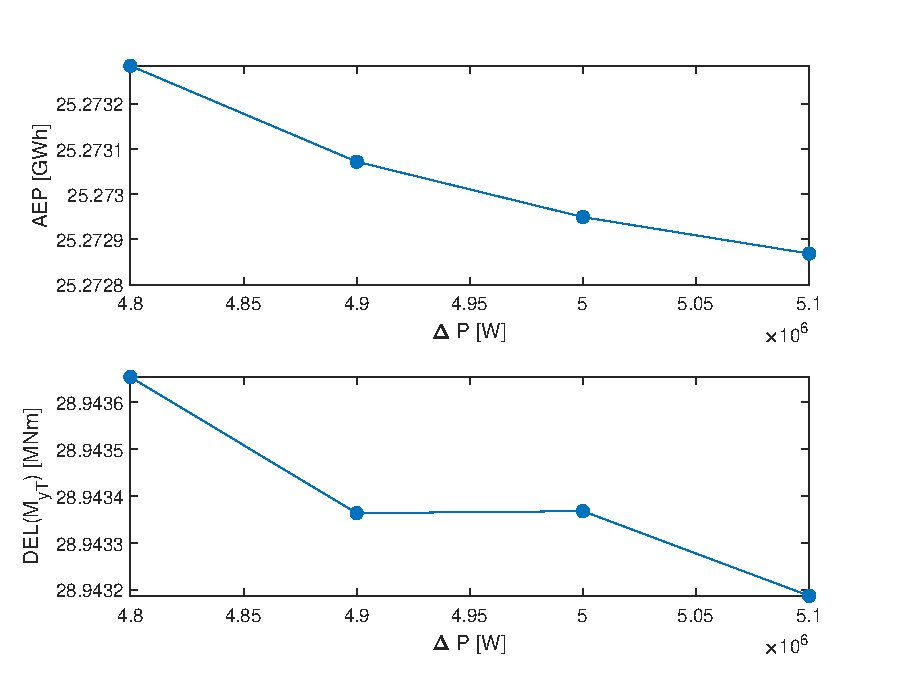
\includegraphics[width=12cm]{Figures/DeltaPopt.eps}
	\caption{Brute-Force optimization of $\Delta P$}
	\label{fig:DeltaP}
\end{figure}

The design value of $k$ is derived first with the help of \ref{eq:k} based on \cite{SchlipfLecture}.
\begin{equation}
	k = \frac{1}{2}\rho\pi R^5 \frac{c_{\text{P,opt}}}{\lambda_{\text{opt}}^3 r_{\text{GB}}^3}
	\label{eq:k}
\end{equation}
The value out of \ref{eq:k} is $k_{\text{design}} = \SI{46.3035}{Nm/(rad/s)^2}$. This is than brute force optimized with a step size of 0.1 as described above.
The resulting value $k$ can next to the other optimized parameters be found in \ref{Control Parameters}. 

The \gls{cpc} gain $kp$ and the gain scheduling parameter $\theta_k$ are effecting not only the \gls{AEP} and the \gls{DEL} of the tower but also the over speed. This introduces another optimization layer. The over speed is computed as \ref{eq:overspeed}. 
\begin{equation}
	\gls{symb:overspeed} = \frac{\hat{\Omega}}{\Omega_{\textnormal{rated}}}
	\label{eq:overspeed}
\end{equation}  
Due to the late design freeze the final \gls{shakti} design leads to low over speeds (less then 10\%). 
A new iterative optimization needs to be done in the future.
The current values are all listed in \ref{Control Parameters}.